% Graphic for TeX using PGF
% Title: /home/budnyjj/univer/GIT/diploma/b/design/diagrams/bl_presenter.dia
% Creator: Dia v0.97.3
% CreationDate: Sun May  8 01:54:36 2016
% For: budnyjj
% \usepackage{tikz}
% The following commands are not supported in PSTricks at present
% We define them conditionally, so when they are implemented,
% this pgf file will use them.
\ifx\du\undefined
  \newlength{\du}
\fi
\setlength{\du}{15\unitlength}
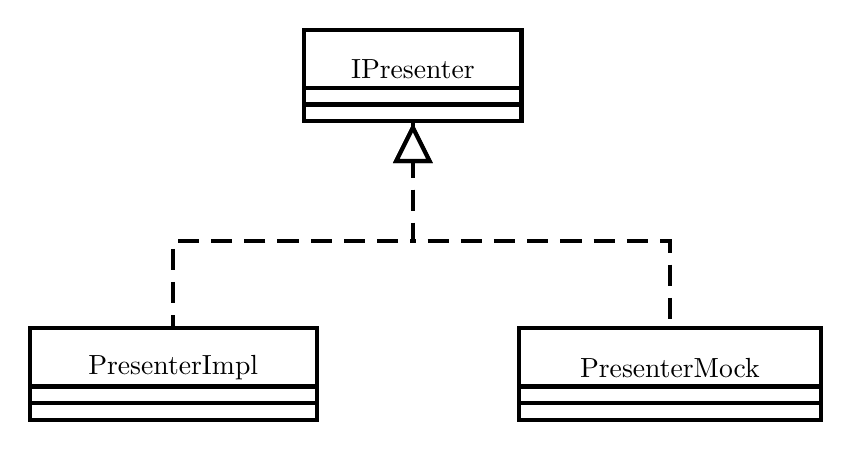
\begin{tikzpicture}
\pgftransformxscale{1.000000}
\pgftransformyscale{-1.000000}
\definecolor{dialinecolor}{rgb}{0.000000, 0.000000, 0.000000}
\pgfsetstrokecolor{dialinecolor}
\definecolor{dialinecolor}{rgb}{1.000000, 1.000000, 1.000000}
\pgfsetfillcolor{dialinecolor}
\pgfsetlinewidth{0.100000\du}
\pgfsetdash{}{0pt}
\definecolor{dialinecolor}{rgb}{1.000000, 1.000000, 1.000000}
\pgfsetfillcolor{dialinecolor}
\fill (25.667770\du,13.261467\du)--(25.667770\du,14.661467\du)--(30.897770\du,14.661467\du)--(30.897770\du,13.261467\du)--cycle;
\definecolor{dialinecolor}{rgb}{0.000000, 0.000000, 0.000000}
\pgfsetstrokecolor{dialinecolor}
\draw (25.667770\du,13.261467\du)--(25.667770\du,14.661467\du)--(30.897770\du,14.661467\du)--(30.897770\du,13.261467\du)--cycle;
% setfont left to latex
\definecolor{dialinecolor}{rgb}{0.000000, 0.000000, 0.000000}
\pgfsetstrokecolor{dialinecolor}
\node at (28.282770\du,14.211467\du){IPresenter};
\definecolor{dialinecolor}{rgb}{1.000000, 1.000000, 1.000000}
\pgfsetfillcolor{dialinecolor}
\fill (25.667770\du,14.661467\du)--(25.667770\du,15.061467\du)--(30.897770\du,15.061467\du)--(30.897770\du,14.661467\du)--cycle;
\definecolor{dialinecolor}{rgb}{0.000000, 0.000000, 0.000000}
\pgfsetstrokecolor{dialinecolor}
\draw (25.667770\du,14.661467\du)--(25.667770\du,15.061467\du)--(30.897770\du,15.061467\du)--(30.897770\du,14.661467\du)--cycle;
\definecolor{dialinecolor}{rgb}{1.000000, 1.000000, 1.000000}
\pgfsetfillcolor{dialinecolor}
\fill (25.667770\du,15.061467\du)--(25.667770\du,15.461467\du)--(30.897770\du,15.461467\du)--(30.897770\du,15.061467\du)--cycle;
\definecolor{dialinecolor}{rgb}{0.000000, 0.000000, 0.000000}
\pgfsetstrokecolor{dialinecolor}
\draw (25.667770\du,15.061467\du)--(25.667770\du,15.461467\du)--(30.897770\du,15.461467\du)--(30.897770\du,15.061467\du)--cycle;
\pgfsetlinewidth{0.100000\du}
\pgfsetdash{}{0pt}
\definecolor{dialinecolor}{rgb}{1.000000, 1.000000, 1.000000}
\pgfsetfillcolor{dialinecolor}
\fill (19.053628\du,20.454747\du)--(19.053628\du,21.854747\du)--(25.963628\du,21.854747\du)--(25.963628\du,20.454747\du)--cycle;
\definecolor{dialinecolor}{rgb}{0.000000, 0.000000, 0.000000}
\pgfsetstrokecolor{dialinecolor}
\draw (19.053628\du,20.454747\du)--(19.053628\du,21.854747\du)--(25.963628\du,21.854747\du)--(25.963628\du,20.454747\du)--cycle;
% setfont left to latex
\definecolor{dialinecolor}{rgb}{0.000000, 0.000000, 0.000000}
\pgfsetstrokecolor{dialinecolor}
\node at (22.508628\du,21.404747\du){PresenterImpl};
\definecolor{dialinecolor}{rgb}{1.000000, 1.000000, 1.000000}
\pgfsetfillcolor{dialinecolor}
\fill (19.053628\du,21.854747\du)--(19.053628\du,22.254747\du)--(25.963628\du,22.254747\du)--(25.963628\du,21.854747\du)--cycle;
\definecolor{dialinecolor}{rgb}{0.000000, 0.000000, 0.000000}
\pgfsetstrokecolor{dialinecolor}
\draw (19.053628\du,21.854747\du)--(19.053628\du,22.254747\du)--(25.963628\du,22.254747\du)--(25.963628\du,21.854747\du)--cycle;
\definecolor{dialinecolor}{rgb}{1.000000, 1.000000, 1.000000}
\pgfsetfillcolor{dialinecolor}
\fill (19.053628\du,22.254747\du)--(19.053628\du,22.654747\du)--(25.963628\du,22.654747\du)--(25.963628\du,22.254747\du)--cycle;
\definecolor{dialinecolor}{rgb}{0.000000, 0.000000, 0.000000}
\pgfsetstrokecolor{dialinecolor}
\draw (19.053628\du,22.254747\du)--(19.053628\du,22.654747\du)--(25.963628\du,22.654747\du)--(25.963628\du,22.254747\du)--cycle;
\pgfsetlinewidth{0.100000\du}
\pgfsetdash{}{0pt}
\definecolor{dialinecolor}{rgb}{1.000000, 1.000000, 1.000000}
\pgfsetfillcolor{dialinecolor}
\fill (30.833541\du,20.454747\du)--(30.833541\du,21.854747\du)--(38.118541\du,21.854747\du)--(38.118541\du,20.454747\du)--cycle;
\definecolor{dialinecolor}{rgb}{0.000000, 0.000000, 0.000000}
\pgfsetstrokecolor{dialinecolor}
\draw (30.833541\du,20.454747\du)--(30.833541\du,21.854747\du)--(38.118541\du,21.854747\du)--(38.118541\du,20.454747\du)--cycle;
% setfont left to latex
\definecolor{dialinecolor}{rgb}{0.000000, 0.000000, 0.000000}
\pgfsetstrokecolor{dialinecolor}
\node at (34.476041\du,21.404747\du){PresenterMock};
\definecolor{dialinecolor}{rgb}{1.000000, 1.000000, 1.000000}
\pgfsetfillcolor{dialinecolor}
\fill (30.833541\du,21.854747\du)--(30.833541\du,22.254747\du)--(38.118541\du,22.254747\du)--(38.118541\du,21.854747\du)--cycle;
\definecolor{dialinecolor}{rgb}{0.000000, 0.000000, 0.000000}
\pgfsetstrokecolor{dialinecolor}
\draw (30.833541\du,21.854747\du)--(30.833541\du,22.254747\du)--(38.118541\du,22.254747\du)--(38.118541\du,21.854747\du)--cycle;
\definecolor{dialinecolor}{rgb}{1.000000, 1.000000, 1.000000}
\pgfsetfillcolor{dialinecolor}
\fill (30.833541\du,22.254747\du)--(30.833541\du,22.654747\du)--(38.118541\du,22.654747\du)--(38.118541\du,22.254747\du)--cycle;
\definecolor{dialinecolor}{rgb}{0.000000, 0.000000, 0.000000}
\pgfsetstrokecolor{dialinecolor}
\draw (30.833541\du,22.254747\du)--(30.833541\du,22.654747\du)--(38.118541\du,22.654747\du)--(38.118541\du,22.254747\du)--cycle;
\pgfsetlinewidth{0.100000\du}
\pgfsetdash{{1.000000\du}{1.000000\du}}{0\du}
\pgfsetdash{{0.400000\du}{0.400000\du}}{0\du}
\pgfsetmiterjoin
\pgfsetbuttcap
{
\definecolor{dialinecolor}{rgb}{0.000000, 0.000000, 0.000000}
\pgfsetfillcolor{dialinecolor}
% was here!!!
\definecolor{dialinecolor}{rgb}{0.000000, 0.000000, 0.000000}
\pgfsetstrokecolor{dialinecolor}
\draw (28.282770\du,15.511747\du)--(28.282770\du,18.358107\du)--(22.508628\du,18.358107\du)--(22.508628\du,20.404466\du);
}
\definecolor{dialinecolor}{rgb}{0.000000, 0.000000, 0.000000}
\pgfsetstrokecolor{dialinecolor}
\draw (28.282770\du,16.423551\du)--(28.282770\du,18.358107\du)--(22.508628\du,18.358107\du)--(22.508628\du,20.404466\du);
\pgfsetmiterjoin
\definecolor{dialinecolor}{rgb}{1.000000, 1.000000, 1.000000}
\pgfsetfillcolor{dialinecolor}
\fill (28.682770\du,16.423551\du)--(28.282770\du,15.623551\du)--(27.882770\du,16.423551\du)--cycle;
\pgfsetlinewidth{0.100000\du}
\pgfsetdash{}{0pt}
\pgfsetmiterjoin
\definecolor{dialinecolor}{rgb}{0.000000, 0.000000, 0.000000}
\pgfsetstrokecolor{dialinecolor}
\draw (28.682770\du,16.423551\du)--(28.282770\du,15.623551\du)--(27.882770\du,16.423551\du)--cycle;
% setfont left to latex
\pgfsetlinewidth{0.100000\du}
\pgfsetdash{{0.400000\du}{0.400000\du}}{0\du}
\pgfsetdash{{0.400000\du}{0.400000\du}}{0\du}
\pgfsetmiterjoin
\pgfsetbuttcap
{
\definecolor{dialinecolor}{rgb}{0.000000, 0.000000, 0.000000}
\pgfsetfillcolor{dialinecolor}
% was here!!!
\definecolor{dialinecolor}{rgb}{0.000000, 0.000000, 0.000000}
\pgfsetstrokecolor{dialinecolor}
\draw (28.282770\du,15.511747\du)--(28.282770\du,18.358107\du)--(34.476041\du,18.358107\du)--(34.476041\du,20.404466\du);
}
\definecolor{dialinecolor}{rgb}{0.000000, 0.000000, 0.000000}
\pgfsetstrokecolor{dialinecolor}
\draw (28.282770\du,16.423551\du)--(28.282770\du,18.358107\du)--(34.476041\du,18.358107\du)--(34.476041\du,20.404466\du);
\pgfsetmiterjoin
\definecolor{dialinecolor}{rgb}{1.000000, 1.000000, 1.000000}
\pgfsetfillcolor{dialinecolor}
\fill (28.682770\du,16.423551\du)--(28.282770\du,15.623551\du)--(27.882770\du,16.423551\du)--cycle;
\pgfsetlinewidth{0.100000\du}
\pgfsetdash{}{0pt}
\pgfsetmiterjoin
\definecolor{dialinecolor}{rgb}{0.000000, 0.000000, 0.000000}
\pgfsetstrokecolor{dialinecolor}
\draw (28.682770\du,16.423551\du)--(28.282770\du,15.623551\du)--(27.882770\du,16.423551\du)--cycle;
% setfont left to latex
\end{tikzpicture}
